\documentclass[12pt]{article}

%packages
%\usepackage{latexsym}
\usepackage{graphicx}
\usepackage{wrapfig}
\usepackage{color}
\usepackage{amsmath}
\usepackage{dsfont}
\usepackage{placeins}
\usepackage{amssymb}
\usepackage{skull}
\usepackage{enumerate}
\usepackage{soul}
\usepackage{alphalph}
\usepackage{hyperref}
\usepackage{enumerate}
\usepackage{listings}
%\usepackage{fancyhdr}

%\fancyhf{} % clear all header and footers
%\renewcommand{\headrulewidth}{0pt} % remove the header rule
%\fancyfoot[LE, LO]{\thepage}


%\usepackage{pstricks,pst-node,pst-tree}

%\usepackage{algpseudocode}
%\usepackage{amsthm}
%\usepackage{hyperref}
%\usepackage{mathrsfs}
%\usepackage{amsfonts}
%\usepackage{bbding}
%\usepackage{listings}
%\usepackage{appendix}
\usepackage[margin=1in]{geometry}
%\geometry{papersize={8.5in,11in},total={6.5in,9in}}
%\usepackage{cancel}
%\usepackage{algorithmic, algorithm}

\definecolor{dkgreen}{rgb}{0,0.6,0}
\definecolor{gray}{rgb}{0.5,0.5,0.5}
\definecolor{mauve}{rgb}{0.58,0,0.82}
\lstset{ %
  language=R,                     % the language of the code
  basicstyle=\footnotesize,       % the size of the fonts that are used for the code
  numbers=left,                   % where to put the line-numbers
  numberstyle=\tiny\color{gray},  % the style that is used for the line-numbers
  stepnumber=1,                   % the step between two line-numbers. If it's 1, each line
                                  % will be numbered
  numbersep=5pt,                  % how far the line-numbers are from the code
  backgroundcolor=\color{white},  % choose the background color. You must add \usepackage{color}
  showspaces=false,               % show spaces adding particular underscores
  showstringspaces=false,         % underline spaces within strings
  showtabs=false,                 % show tabs within strings adding particular underscores
  frame=single,                   % adds a frame around the code
  rulecolor=\color{black},        % if not set, the frame-color may be changed on line-breaks within not-black text (e.g. commens (green here))
  tabsize=2,                      % sets default tabsize to 2 spaces
  captionpos=b,                   % sets the caption-position to bottom
  breaklines=true,                % sets automatic line breaking
  breakatwhitespace=false,        % sets if automatic breaks should only happen at whitespace
  title=\lstname,                 % show the filename of files included with \lstinputlisting;
                                  % also try caption instead of title
  keywordstyle=\color{blue},      % keyword style
  commentstyle=\color{dkgreen},   % comment style
  stringstyle=\color{mauve},      % string literal style
  escapeinside={\%*}{*)},         % if you want to add a comment within your code
  morekeywords={*,...}            % if you want to add more keywords to the set
}

\newcommand{\qu}[1]{``#1''}
\newcommand{\spc}[1]{\\ \vspace{#1cm}}

\newcounter{probnum}
\setcounter{probnum}{1}
\newcounter{numpts}
\setcounter{numpts}{0}

%create definition to allow local margin changes
\def\changemargin#1#2{\list{}{\rightmargin#2\leftmargin#1}\item[]}
\let\endchangemargin=\endlist 

%allow equations to span multiple pages
\allowdisplaybreaks

%define colors and color typesetting conveniences
\definecolor{gray}{rgb}{0.5,0.5,0.5}
\definecolor{black}{rgb}{0,0,0}
\definecolor{white}{rgb}{1,1,1}
\definecolor{blue}{rgb}{0.5,0.5,1}
\newcommand{\inblue}[1]{\color{blue}#1 \color{black}}
\definecolor{green}{rgb}{0.133,0.545,0.133}
\newcommand{\ingreen}[1]{\color{green}#1 \color{black}}
\definecolor{yellow}{rgb}{1,0.549,0}
\newcommand{\inyellow}[1]{\color{yellow}#1 \color{black}}
\definecolor{red}{rgb}{1,0.133,0.133}
\newcommand{\inred}[1]{\color{red}#1 \color{black}}
\definecolor{purple}{rgb}{0.58,0,0.827}
\newcommand{\inpurple}[1]{\color{purple}#1 \color{black}}
\definecolor{gray}{rgb}{0.5,0.5,0.5}
\newcommand{\ingray}[1]{\color{gray}#1 \color{black}}
\definecolor{backgcode}{rgb}{0.97,0.97,0.8}
\definecolor{Brown}{cmyk}{0,0.81,1,0.60}
\definecolor{OliveGreen}{cmyk}{0.64,0,0.95,0.40}
\definecolor{CadetBlue}{cmyk}{0.62,0.57,0.23,0}

%define new math operators
\DeclareMathOperator*{\argmax}{arg\,max~}
\DeclareMathOperator*{\argmin}{arg\,min~}
\DeclareMathOperator*{\argsup}{arg\,sup~}
\DeclareMathOperator*{\arginf}{arg\,inf~}
\DeclareMathOperator*{\convolution}{\text{\Huge{$\ast$}}}
\newcommand{\infconv}[2]{\convolution^\infty_{#1 = 1} #2}
%true functions

%%%% GENERAL SHORTCUTS

\makeatletter
\newalphalph{\alphmult}[mult]{\@alph}{26}
\renewcommand{\labelenumi}{(\alphmult{\value{enumi}})}
\renewcommand{\theenumi}{\AlphAlph{\value{enumi}}}
\makeatother
%shortcuts for pure typesetting conveniences
\newcommand{\bv}[1]{\boldsymbol{#1}}

%shortcuts for compound constants
\newcommand{\BetaDistrConst}{\dfrac{\Gamma(\alpha + \beta)}{\Gamma(\alpha)\Gamma(\beta)}}
\newcommand{\NormDistrConst}{\dfrac{1}{\sqrt{2\pi\sigma^2}}}

%shortcuts for conventional symbols
\newcommand{\tsq}{\tau^2}
\newcommand{\tsqh}{\hat{\tau}^2}
\newcommand{\sigsq}{\sigma^2}
\newcommand{\sigsqsq}{\parens{\sigma^2}^2}
\newcommand{\sigsqovern}{\dfrac{\sigsq}{n}}
\newcommand{\tausq}{\tau^2}
\newcommand{\tausqalpha}{\tau^2_\alpha}
\newcommand{\tausqbeta}{\tau^2_\beta}
\newcommand{\tausqsigma}{\tau^2_\sigma}
\newcommand{\betasq}{\beta^2}
\newcommand{\sigsqvec}{\bv{\sigma}^2}
\newcommand{\sigsqhat}{\hat{\sigma}^2}
\newcommand{\sigsqhatmlebayes}{\sigsqhat_{\text{Bayes, MLE}}}
\newcommand{\sigsqhatmle}[1]{\sigsqhat_{#1, \text{MLE}}}
\newcommand{\bSigma}{\bv{\Sigma}}
\newcommand{\bSigmainv}{\bSigma^{-1}}
\newcommand{\thetavec}{\bv{\theta}}
\newcommand{\thetahat}{\hat{\theta}}
\newcommand{\thetahatmle}{\hat{\theta}_{\mathrm{MLE}}}
\newcommand{\thetavechatmle}{\hat{\thetavec}_{\mathrm{MLE}}}
\newcommand{\muhat}{\hat{\mu}}
\newcommand{\musq}{\mu^2}
\newcommand{\muvec}{\bv{\mu}}
\newcommand{\muhatmle}{\muhat_{\text{MLE}}}
\newcommand{\lambdahat}{\hat{\lambda}}
\newcommand{\lambdahatmle}{\lambdahat_{\text{MLE}}}
\newcommand{\thetahatmap}{\hat{\theta}_{\mathrm{MAP}}}
\newcommand{\thetahatmae}{\hat{\theta}_{\mathrm{MAE}}}
\newcommand{\thetahatmmse}{\hat{\theta}_{\mathrm{MMSE}}}
\newcommand{\etavec}{\bv{\eta}}
\newcommand{\alphavec}{\bv{\alpha}}
\newcommand{\minimaxdec}{\delta^*_{\mathrm{mm}}}
\newcommand{\ybar}{\bar{y}}
\newcommand{\xbar}{\bar{x}}
\newcommand{\Xbar}{\bar{X}}
\newcommand{\iid}{~{\buildrel iid \over \sim}~}
\newcommand{\inddist}{~{\buildrel ind \over \sim}~}
\newcommand{\approxdist}{~{\buildrel approx \over \sim}~}
\newcommand{\equalsindist}{~{\buildrel d \over =}~}
\newcommand{\loglik}[1]{\ell\parens{#1}}
\newcommand{\thetahatkminone}{\thetahat^{(k-1)}}
\newcommand{\thetahatkplusone}{\thetahat^{(k+1)}}
\newcommand{\thetahatk}{\thetahat^{(k)}}
\newcommand{\half}{\frac{1}{2}}
\newcommand{\third}{\frac{1}{3}}
\newcommand{\twothirds}{\frac{2}{3}}
\newcommand{\fourth}{\frac{1}{4}}
\newcommand{\fifth}{\frac{1}{5}}
\newcommand{\sixth}{\frac{1}{6}}

%shortcuts for vector and matrix notation
\newcommand{\A}{\bv{A}}
\newcommand{\At}{\A^T}
\renewcommand{\H}{\bv{H}}
\newcommand{\Ht}{\H^\top}
\newcommand{\Ainv}{\inverse{\A}}
\newcommand{\B}{\bv{B}}
\newcommand{\K}{\bv{K}}
\newcommand{\Kt}{\K^T}
\newcommand{\Kinv}{\inverse{K}}
\newcommand{\Kinvt}{(\Kinv)^T}
\newcommand{\M}{\bv{M}}
\newcommand{\Bt}{\B^T}
\newcommand{\Q}{\bv{Q}}
\newcommand{\Qt}{\Q^T}
\newcommand{\R}{\bv{R}}
\newcommand{\Rt}{\R^T}
\newcommand{\Z}{\bv{Z}}
\newcommand{\X}{\bv{X}}
\renewcommand{\b}{\bv{b}}
\newcommand{\Xsub}{\X_{\text{(sub)}}}
\newcommand{\Xsubadj}{\X_{\text{(sub,adj)}}}
\newcommand{\I}{\bv{I}}
\newcommand{\Y}{\bv{Y}}
\newcommand{\sigsqI}{\sigsq\I}
\renewcommand{\P}{\bv{P}}
\newcommand{\Psub}{\P_{\text{(sub)}}}
\newcommand{\Pt}{\P^T}
\newcommand{\Pii}{P_{ii}}
\newcommand{\Pij}{P_{ij}}
\newcommand{\IminP}{(\I-\P)}
\newcommand{\Xt}{\bv{X}^T}
\newcommand{\XtX}{\Xt\X}
\newcommand{\XtXinv}{\parens{\Xt\X}^{-1}}
\newcommand{\XtXinvXt}{\XtXinv\Xt}
\newcommand{\XXtXinvXt}{\X\XtXinvXt}
\newcommand{\x}{\bv{x}}
\newcommand{\w}{\bv{w}}
\newcommand{\onevec}{\bv{1}}
\newcommand{\oneton}{1, \ldots, n}
\newcommand{\yoneton}{y_1, \ldots, y_n}
\newcommand{\yonetonorder}{y_{(1)}, \ldots, y_{(n)}}
\newcommand{\Yoneton}{Y_1, \ldots, Y_n}
\newcommand{\iinoneton}{i \in \braces{\oneton}}
\newcommand{\onetom}{1, \ldots, m}
\newcommand{\jinonetom}{j \in \braces{\onetom}}
\newcommand{\xoneton}{x_1, \ldots, x_n}
\newcommand{\Xoneton}{X_1, \ldots, X_n}
\newcommand{\xt}{\x^T}
\newcommand{\y}{\bv{y}}
\newcommand{\yt}{\y^T}
\renewcommand{\c}{\bv{c}}
\newcommand{\ct}{\c^T}
\newcommand{\tstar}{\bv{t}^*}
\renewcommand{\u}{\bv{u}}
\renewcommand{\v}{\bv{v}}
\renewcommand{\a}{\bv{a}}
\newcommand{\s}{\bv{s}}
\newcommand{\yadj}{\y_{\text{(adj)}}}
\newcommand{\xjadj}{\x_{j\text{(adj)}}}
\newcommand{\xjadjM}{\x_{j \perp M}}
\newcommand{\yhat}{\hat{\y}}
\newcommand{\yhatsub}{\yhat_{\text{(sub)}}}
\newcommand{\yhatstar}{\yhat^*}
\newcommand{\yhatstarnew}{\yhatstar_{\text{new}}}
\newcommand{\z}{\bv{z}}
\newcommand{\zt}{\z^T}
\newcommand{\bb}{\bv{b}}
\newcommand{\bbt}{\bb^T}
\newcommand{\bbeta}{\bv{\beta}}
\newcommand{\beps}{\bv{\epsilon}}
\newcommand{\bepst}{\beps^T}
\newcommand{\e}{\bv{e}}
\newcommand{\Mofy}{\M(\y)}
\newcommand{\KofAlpha}{K(\alpha)}
\newcommand{\ellset}{\mathcal{L}}
\newcommand{\oneminalph}{1-\alpha}
\newcommand{\SSE}{\text{SSE}}
\newcommand{\SSEsub}{\text{SSE}_{\text{(sub)}}}
\newcommand{\MSE}{\text{MSE}}
\newcommand{\RMSE}{\text{RMSE}}
\newcommand{\SSR}{\text{SSR}}
\newcommand{\SST}{\text{SST}}
\newcommand{\JSest}{\delta_{\text{JS}}(\x)}
\newcommand{\Bayesest}{\delta_{\text{Bayes}}(\x)}
\newcommand{\EmpBayesest}{\delta_{\text{EmpBayes}}(\x)}
\newcommand{\BLUPest}{\delta_{\text{BLUP}}}
\newcommand{\MLEest}[1]{\hat{#1}_{\text{MLE}}}

%shortcuts for Linear Algebra stuff (i.e. vectors and matrices)
\newcommand{\twovec}[2]{\bracks{\begin{array}{c} #1 \\ #2 \end{array}}}
\newcommand{\threevec}[3]{\bracks{\begin{array}{c} #1 \\ #2 \\ #3 \end{array}}}
\newcommand{\fivevec}[5]{\bracks{\begin{array}{c} #1 \\ #2 \\ #3 \\ #4 \\ #5 \end{array}}}
\newcommand{\twobytwomat}[4]{\bracks{\begin{array}{cc} #1 & #2 \\ #3 & #4 \end{array}}}
\newcommand{\threebytwomat}[6]{\bracks{\begin{array}{cc} #1 & #2 \\ #3 & #4 \\ #5 & #6 \end{array}}}

%shortcuts for conventional compound symbols
\newcommand{\thetainthetas}{\theta \in \Theta}
\newcommand{\reals}{\mathbb{R}}
\newcommand{\complexes}{\mathbb{C}}
\newcommand{\rationals}{\mathbb{Q}}
\newcommand{\integers}{\mathbb{Z}}
\newcommand{\naturals}{\mathbb{N}}
\newcommand{\forallninN}{~~\forall n \in \naturals}
\newcommand{\forallxinN}[1]{~~\forall #1 \in \reals}
\newcommand{\matrixdims}[2]{\in \reals^{\,#1 \times #2}}
\newcommand{\inRn}[1]{\in \reals^{\,#1}}
\newcommand{\mathimplies}{\quad\Rightarrow\quad}
\newcommand{\mathlogicequiv}{\quad\Leftrightarrow\quad}
\newcommand{\eqncomment}[1]{\quad \text{(#1)}}
\newcommand{\limitn}{\lim_{n \rightarrow \infty}}
\newcommand{\limitN}{\lim_{N \rightarrow \infty}}
\newcommand{\limitd}{\lim_{d \rightarrow \infty}}
\newcommand{\limitt}{\lim_{t \rightarrow \infty}}
\newcommand{\limitsupn}{\limsup_{n \rightarrow \infty}~}
\newcommand{\limitinfn}{\liminf_{n \rightarrow \infty}~}
\newcommand{\limitk}{\lim_{k \rightarrow \infty}}
\newcommand{\limsupn}{\limsup_{n \rightarrow \infty}}
\newcommand{\limsupk}{\limsup_{k \rightarrow \infty}}
\newcommand{\floor}[1]{\left\lfloor #1 \right\rfloor}
\newcommand{\ceil}[1]{\left\lceil #1 \right\rceil}

%shortcuts for environments
\newcommand{\beqn}{\vspace{-0.25cm}\begin{eqnarray*}}
\newcommand{\eeqn}{\end{eqnarray*}}
\newcommand{\bneqn}{\vspace{-0.25cm}\begin{eqnarray}}
\newcommand{\eneqn}{\end{eqnarray}}
\newcommand{\benum}{\begin{enumerate}}
\newcommand{\eenum}{\end{enumerate}}

%shortcuts for mini environments
\newcommand{\parens}[1]{\left(#1\right)}
\newcommand{\squared}[1]{\parens{#1}^2}
\newcommand{\tothepow}[2]{\parens{#1}^{#2}}
\newcommand{\prob}[1]{\mathbb{P}\parens{#1}}
\newcommand{\littleo}[1]{o\parens{#1}}
\newcommand{\bigo}[1]{O\parens{#1}}
\newcommand{\Lp}[1]{\mathbb{L}^{#1}}
\renewcommand{\arcsin}[1]{\text{arcsin}\parens{#1}}
\newcommand{\prodonen}[2]{\bracks{\prod_{#1=1}^n #2}}
\newcommand{\mysum}[4]{\sum_{#1=#2}^{#3} #4}
\newcommand{\sumonen}[2]{\sum_{#1=1}^n #2}
\newcommand{\infsum}[2]{\sum_{#1=1}^\infty #2}
\newcommand{\infprod}[2]{\prod_{#1=1}^\infty #2}
\newcommand{\infunion}[2]{\bigcup_{#1=1}^\infty #2}
\newcommand{\infinter}[2]{\bigcap_{#1=1}^\infty #2}
\newcommand{\infintegral}[2]{\int^\infty_{-\infty} #2 ~\text{d}#1}
\newcommand{\supthetas}[1]{\sup_{\thetainthetas}\braces{#1}}
\newcommand{\bracks}[1]{\left[#1\right]}
\newcommand{\braces}[1]{\left\{#1\right\}}
\newcommand{\set}[1]{\left\{#1\right\}}
\newcommand{\abss}[1]{\left|#1\right|}
\newcommand{\norm}[1]{\left|\left|#1\right|\right|}
\newcommand{\normsq}[1]{\norm{#1}^2}
\newcommand{\inverse}[1]{\parens{#1}^{-1}}
\newcommand{\rowof}[2]{\parens{#1}_{#2\cdot}}

%shortcuts for functionals
\newcommand{\realcomp}[1]{\text{Re}\bracks{#1}}
\newcommand{\imagcomp}[1]{\text{Im}\bracks{#1}}
\newcommand{\range}[1]{\text{range}\bracks{#1}}
\newcommand{\colsp}[1]{\text{colsp}\bracks{#1}}
\newcommand{\rowsp}[1]{\text{rowsp}\bracks{#1}}
\newcommand{\tr}[1]{\text{tr}\bracks{#1}}
\newcommand{\rank}[1]{\text{rank}\bracks{#1}}
\newcommand{\proj}[2]{\text{Proj}_{#1}\bracks{#2}}
\newcommand{\projcolspX}[1]{\text{Proj}_{\colsp{\X}}\bracks{#1}}
\newcommand{\median}[1]{\text{median}\bracks{#1}}
\newcommand{\mean}[1]{\text{mean}\bracks{#1}}
\newcommand{\dime}[1]{\text{dim}\bracks{#1}}
\renewcommand{\det}[1]{\text{det}\bracks{#1}}
\newcommand{\expe}[1]{\mathbb{E}\bracks{#1}}
\newcommand{\expeabs}[1]{\expe{\abss{#1}}}
\newcommand{\expesub}[2]{\mathbb{E}_{#1}\bracks{#2}}
\newcommand{\cexpesub}[3]{\mathbb{E}_{#1}\bracks{#2~|~#3}}
\newcommand{\indic}[1]{\mathds{1}_{#1}}
\newcommand{\var}[1]{\mathbb{V}\text{ar}\bracks{#1}}
\newcommand{\sd}[1]{\mathbb{S}\text{D}\bracks{#1}}
\newcommand{\cov}[2]{\text{Cov}\bracks{#1, #2}}
\newcommand{\corr}[2]{\text{Corr}\bracks{#1, #2}}
\newcommand{\se}[1]{\text{SE}\bracks{#1}}
\newcommand{\seest}[1]{\hat{\text{SE}}\bracks{#1}}
\newcommand{\bias}[1]{\text{Bias}\bracks{#1}}
\newcommand{\partialop}[2]{\dfrac{\partial}{\partial #1}\bracks{#2}}
\newcommand{\secpartialop}[2]{\dfrac{\partial^2}{\partial #1^2}\bracks{#2}}
\newcommand{\mixpartialop}[3]{\dfrac{\partial^2}{\partial #1 \partial #2}\bracks{#3}}

%shortcuts for functions
\renewcommand{\exp}[1]{\mathrm{exp}\parens{#1}}
\renewcommand{\cos}[1]{\text{cos}\parens{#1}}
\renewcommand{\sin}[1]{\text{sin}\parens{#1}}
\newcommand{\sign}[1]{\text{sign}\parens{#1}}
\newcommand{\are}[1]{\mathrm{ARE}\parens{#1}}
\newcommand{\natlog}[1]{\ln\parens{#1}}
\newcommand{\oneover}[1]{\frac{1}{#1}}
\newcommand{\overtwo}[1]{\frac{#1}{2}}
\newcommand{\overn}[1]{\frac{#1}{n}}
\newcommand{\oneoversqrt}[1]{\oneover{\sqrt{#1}}}
\newcommand{\sqd}[1]{\parens{#1}^2}
\newcommand{\loss}[1]{\ell\parens{\theta, #1}}
\newcommand{\losstwo}[2]{\ell\parens{#1, #2}}
\newcommand{\cf}{\phi(t)}

%English language specific shortcuts
\newcommand{\ie}{\textit{i.e.} }
\newcommand{\AKA}{\textit{AKA} }
\renewcommand{\iff}{\textit{iff}}
\newcommand{\eg}{\textit{e.g.} }
\renewcommand{\st}{\textit{s.t.} }
\newcommand{\wrt}{\textit{w.r.t.} }
\newcommand{\mathst}{~~\text{\st}~~}
\newcommand{\mathand}{~~\text{and}~~}
\newcommand{\ala}{\textit{a la} }
\newcommand{\ppp}{posterior predictive p-value}
\newcommand{\dd}{dataset-to-dataset}

%shortcuts for distribution titles
\newcommand{\logistic}[2]{\mathrm{Logistic}\parens{#1,\,#2}}
\newcommand{\bernoulli}[1]{\mathrm{Bernoulli}\parens{#1}}
\newcommand{\betanot}[2]{\mathrm{Beta}\parens{#1,\,#2}}
\newcommand{\stdbetanot}{\betanot{\alpha}{\beta}}
\newcommand{\multnormnot}[3]{\mathcal{N}_{#1}\parens{#2,\,#3}}
\newcommand{\normnot}[2]{\mathcal{N}\parens{#1,\,#2}}
\newcommand{\classicnormnot}{\normnot{\mu}{\sigsq}}
\newcommand{\stdnormnot}{\normnot{0}{1}}
\newcommand{\uniform}[2]{\mathrm{U}\parens{#1,\,#2}}
\newcommand{\stduniform}{\uniform{0}{1}}
\newcommand{\exponential}[1]{\mathrm{Exp}\parens{#1}}
\newcommand{\gammadist}[2]{\mathrm{Gamma}\parens{#1, #2}}
\newcommand{\poisson}[1]{\mathrm{Poisson}\parens{#1}}
\newcommand{\binomial}[2]{\mathrm{Binomial}\parens{#1,\,#2}}
\newcommand{\rayleigh}[1]{\mathrm{Rayleigh}\parens{#1}}
\newcommand{\multinomial}[2]{\mathrm{Multinomial}\parens{#1,\,#2}}
\newcommand{\gammanot}[2]{\mathrm{Gamma}\parens{#1,\,#2}}
\newcommand{\cauchynot}[2]{\text{Cauchy}\parens{#1,\,#2}}
\newcommand{\invchisqnot}[1]{\text{Inv}\chisq{#1}}
\newcommand{\invscaledchisqnot}[2]{\text{ScaledInv}\ncchisq{#1}{#2}}
\newcommand{\invgammanot}[2]{\text{InvGamma}\parens{#1,\,#2}}
\newcommand{\chisq}[1]{\chi^2_{#1}}
\newcommand{\ncchisq}[2]{\chi^2_{#1}\parens{#2}}
\newcommand{\ncF}[3]{F_{#1,#2}\parens{#3}}

%shortcuts for PDF's of common distributions
\newcommand{\logisticpdf}[3]{\oneover{#3}\dfrac{\exp{-\dfrac{#1 - #2}{#3}}}{\parens{1+\exp{-\dfrac{#1 - #2}{#3}}}^2}}
\newcommand{\betapdf}[3]{\dfrac{\Gamma(#2 + #3)}{\Gamma(#2)\Gamma(#3)}#1^{#2-1} (1-#1)^{#3-1}}
\newcommand{\normpdf}[3]{\frac{1}{\sqrt{2\pi#3}}\exp{-\frac{1}{2#3}(#1 - #2)^2}}
\newcommand{\normpdfvarone}[2]{\dfrac{1}{\sqrt{2\pi}}e^{-\half(#1 - #2)^2}}
\newcommand{\chisqpdf}[2]{\dfrac{1}{2^{#2/2}\Gamma(#2/2)}\; {#1}^{#2/2-1} e^{-#1/2}}
\newcommand{\invchisqpdf}[2]{\dfrac{2^{-\overtwo{#1}}}{\Gamma(#2/2)}\,{#1}^{-\overtwo{#2}-1}  e^{-\oneover{2 #1}}}
\newcommand{\uniformdiscrete}[1]{\mathrm{Uniform}\parens{\braces{#1}}}
\newcommand{\exponentialpdf}[2]{#2\exp{-#2#1}}
\newcommand{\poissonpdf}[2]{\dfrac{e^{-#1} #1^{#2}}{#2!}}
\newcommand{\binomialpdf}[3]{\binom{#2}{#1}#3^{#1}(1-#3)^{#2-#1}}
\newcommand{\rayleighpdf}[2]{\dfrac{#1}{#2^2}\exp{-\dfrac{#1^2}{2 #2^2}}}
\newcommand{\gammapdf}[3]{\dfrac{#3^#2}{\Gamma\parens{#2}}#1^{#2-1}\exp{-#3 #1}}
\newcommand{\cauchypdf}[3]{\oneover{\pi} \dfrac{#3}{\parens{#1-#2}^2 + #3^2}}
\newcommand{\Gammaf}[1]{\Gamma\parens{#1}}

%shortcuts for miscellaneous typesetting conveniences
\newcommand{\notesref}[1]{\marginpar{\color{gray}\tt #1\color{black}}}

%%%% DOMAIN-SPECIFIC SHORTCUTS

%Real analysis related shortcuts
\newcommand{\zeroonecl}{\bracks{0,1}}
\newcommand{\forallepsgrzero}{\forall \epsilon > 0~~}
\newcommand{\lessthaneps}{< \epsilon}
\newcommand{\fraccomp}[1]{\text{frac}\bracks{#1}}

%Bayesian related shortcuts
\newcommand{\yrep}{y^{\text{rep}}}
\newcommand{\yrepisq}{(\yrep_i)^2}
\newcommand{\yrepvec}{\bv{y}^{\text{rep}}}


%Probability shortcuts
\newcommand{\SigField}{\mathcal{F}}
\newcommand{\ProbMap}{\mathcal{P}}
\newcommand{\probtrinity}{\parens{\Omega, \SigField, \ProbMap}}
\newcommand{\convp}{~{\buildrel p \over \rightarrow}~}
\newcommand{\convLp}[1]{~{\buildrel \Lp{#1} \over \rightarrow}~}
\newcommand{\nconvp}{~{\buildrel p \over \nrightarrow}~}
\newcommand{\convae}{~{\buildrel a.e. \over \longrightarrow}~}
\newcommand{\convau}{~{\buildrel a.u. \over \longrightarrow}~}
\newcommand{\nconvau}{~{\buildrel a.u. \over \nrightarrow}~}
\newcommand{\nconvae}{~{\buildrel a.e. \over \nrightarrow}~}
\newcommand{\convd}{~{\buildrel \mathcal{D} \over \rightarrow}~}
\newcommand{\nconvd}{~{\buildrel \mathcal{D} \over \nrightarrow}~}
\newcommand{\withprob}{~~\text{w.p.}~~}
\newcommand{\io}{~~\text{i.o.}}

\newcommand{\Acl}{\bar{A}}
\newcommand{\ENcl}{\bar{E}_N}
\newcommand{\diam}[1]{\text{diam}\parens{#1}}

\newcommand{\taua}{\tau_a}

\newcommand{\myint}[4]{\int_{#2}^{#3} #4 \,\text{d}#1}
\newcommand{\laplacet}[1]{\mathscr{L}\bracks{#1}}
\newcommand{\laplaceinvt}[1]{\mathscr{L}^{-1}\bracks{#1}}
\renewcommand{\min}[1]{\text{min}\braces{#1}}

\newcommand{\Vbar}[1]{\bar{V}\parens{#1}}
\newcommand{\expnegrtau}{\exp{-r\tau}}
\newcommand{\cprob}[2]{\prob{#1~|~#2}}

%%% problem typesetting
\newcommand{\problem}{\vspace{0.2cm} \noindent {\large{\textsf{Problem \arabic{probnum}~}}} \addtocounter{probnum}{1}}
%\newcommand{\easyproblem}{\ingreen{\noindent \textsf{Problem \arabic{probnum}~}} \addtocounter{probnum}{1}}
%\newcommand{\intermediateproblem}{\noindent \inyellow{\textsf{Problem \arabic{probnum}~}} \addtocounter{probnum}{1}}
%\newcommand{\hardproblem}{\inred{\noindent \textsf{Problem \arabic{probnum}~}} \addtocounter{probnum}{1}}
%\newcommand{\extracreditproblem}{\noindent \inpurple{\textsf{Problem \arabic{probnum}~}} \addtocounter{probnum}{1}}

\newcommand{\easysubproblem}{\ingreen{\item}}
\newcommand{\intermediatesubproblem}{\inyellow{\item}}
\newcommand{\hardsubproblem}{\inred{\item}}
\newcommand{\extracreditsubproblem}{\inpurple{\item}}
%\newcommand{\subquestionwithpoints}[1]{\addtocounter{numpts}{#1} \item \ingray{[#1 pt]}~~} %  / \arabic{numpts} pts
\newcommand{\subquestionwithpoints}[1]{\addtocounter{numpts}{#1} \item \ingray{[#1 pt / \arabic{numpts} pts]}~~}  

\title{Math 390.4 / 650.3 Spring 2018 \\ Final Examination}
\author{Professor Adam Kapelner}

\date{Wednesday, May 23, 2018}

\begin{document}
\maketitle

\noindent Full Name \line(1,0){410}

\thispagestyle{empty}

\section*{Code of Academic Integrity}

\footnotesize
Since the college is an academic community, its fundamental purpose is the pursuit of knowledge. Essential to the success of this educational mission is a commitment to the principles of academic integrity. Every member of the college community is responsible for upholding the highest standards of honesty at all times. Students, as members of the community, are also responsible for adhering to the principles and spirit of the following Code of Academic Integrity.

Activities that have the effect or intention of interfering with education, pursuit of knowledge, or fair evaluation of a student's performance are prohibited. Examples of such activities include but are not limited to the following definitions:

\paragraph{Cheating} Using or attempting to use unauthorized assistance, material, or study aids in examinations or other academic work or preventing, or attempting to prevent, another from using authorized assistance, material, or study aids. Example: using an unauthorized cheat sheet in a quiz or exam, altering a graded exam and resubmitting it for a better grade, etc.
\\

\noindent I acknowledge and agree to uphold this Code of Academic Integrity. \\

\begin{center}
\line(1,0){250} ~~~ \line(1,0){100}\\
~~~~~~~~~~~~~~~~~~~~~signature~~~~~~~~~~~~~~~~~~~~~~~~~~~~~~~~~~~~~~~~~~~~~ date
\end{center}

\normalsize

\section*{Instructions}

This exam is 120 minutes and closed-book. You are allowed \textbf{three} pages (front and back) of a \qu{cheat sheet.} You may use a graphing calculator of your choice. Please read the questions carefully. If the question reads \qu{compute,} this means the solution will be a number otherwise you can leave the answer in \textit{any} widely accepted mathematical notation which could be resolved to an exact or approximate number with the use of a computer. I advise you to skip problems marked \qu{[Extra Credit]} until you have finished the other questions on the exam, then loop back and plug in all the holes. I also advise you to use pencil. The exam is 100 points total plus extra credit. Partial credit will be granted for incomplete answers on most of the questions. \fbox{Box} in your final answers. Good luck!

\pagebreak


\problem This question is about the theory of modeling through the ideas introduced in the class readings.

\benum

\subquestionwithpoints{2} Write the bias-variance decomposition for the oos MSE of a model $g$ averaged over the distribution of the ignorance $\Delta$ and the covariate space $\mathcal{X}$.\spc{4}

\subquestionwithpoints{5} Chapter 5 in Nate Silver's book \qu{The Signal and the Noise} is all about predicting earthquake magnitudes of which large magnitudes are destructive and sometimes fatal. Broadly speaking, what is the problem with predicting when large earthquakes will occur? Make sure you use the framework and notation from class especially the bias-variance decomposition from (a). There is no \qu{right} answer; thus, you will be graded on your ability to construct arguments and tie your reasoning to the concepts from class. \spc{15}

%\subquestionwithpoints{4} [Extra Credit] Chapter 4 in Nate Silver's book \qu{The Signal and the Noise} is all about predicting weather. Broadly speaking, what is the problem with weather predictions? Make sure you use the framework and notation from class. There is no \qu{right} answer; thus, you will be graded on your ability to construct arguments and tie your reasoning to the concepts from class. \spc{10}



\eenum


\problem In the homework we discussed the OLS estimator and the ridge estimator:

\beqn
\b_{OLS} = \XtXinv\Xt\y \quad\mathand\quad \b_{ridge} = \inverse{\XtX + \lambda\I_{p+1}}\Xt\y \quad \text{where}~ \lambda > 0
\eeqn

\noindent This question deals with questions about these models.

\benum

\subquestionwithpoints{5} Let's say you are building both (I) an OLS model and (II) a ridge model with $\lambda = 0.32$ with the same data. Circle all thing(s) that are different between these two models.


\begin{enumerate}[i)]
\item $\XtX$
\item $p$
\item $\mathcal{Y}$
\item $\mathbb{D}$
\item $\mathcal{H}$
\item $\mathcal{A}$
\item the degrees of freedom
\item $\b$
\item $g$
\item $f$
\item $\yhat$
\item the validation procedure to assess generalizability of the model
\item the value of $K$ in $K$-fold CV
\item the new observation $\x^*$ whose $y^*$ we will predict
\item the oos error
\end{enumerate}


\subquestionwithpoints{2} Let's say you are building both an OLS and a ridge model with $\lambda = 0.32$ where $n < p + 1$, circle all true statements:

\begin{enumerate}[i)]
\item $\norm{\b_{OLS}} < \norm{\b_{ridge}}$
\item $\norm{\b_{OLS}} = \norm{\b_{ridge}}$
\item $\norm{\b_{OLS}} > \norm{\b_{ridge}}$
\item None of the above.
\end{enumerate}
\clearpage

\subquestionwithpoints{2} Let's say you are building both an OLS and a ridge model with $\lambda = 0.32$ where $n > p + 1$, circle all true statements:

\begin{enumerate}[i)]
\item $\norm{\b_{OLS}} < \norm{\b_{ridge}}$
\item $\norm{\b_{OLS}} = \norm{\b_{ridge}}$
\item $\norm{\b_{OLS}} > \norm{\b_{ridge}}$
\item None of the above.
\end{enumerate}


\subquestionwithpoints{4} Let's say you want to build a ridge model, but you don't know which $\lambda$ to pick. Describe an algorithm below that picks $\lambda$ and explain clearly on what basis you are picking $\lambda$. \spc{9}

\subquestionwithpoints{4} [Extra Credit] If $\lambda \rightarrow \infty$, reason that $\b_{ridge} \rightarrow \zerovec_{p+1}$. \spc{10}


\subquestionwithpoints{3} Is ridge regression \qu{non-parametric}? Yes /no and explain. \spc{5}
\eenum


\problem Consider the following illustration:

\begin{figure}[htp]
\centering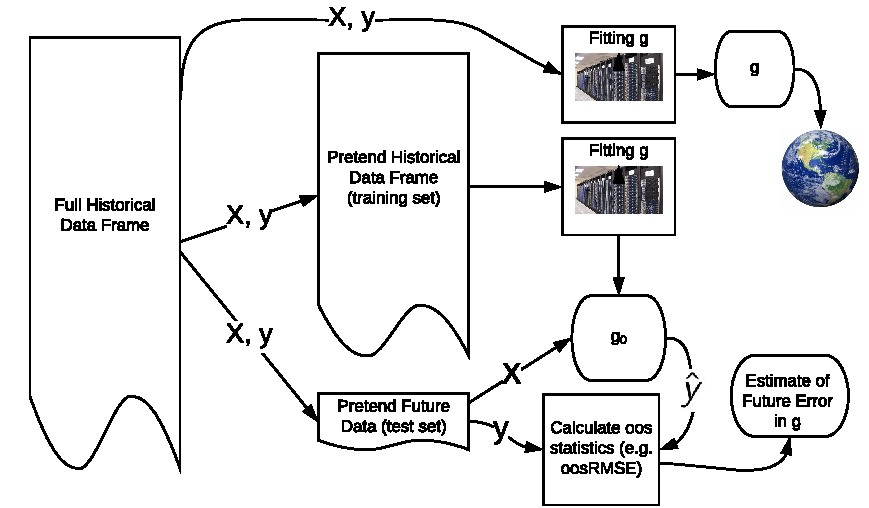
\includegraphics[width=7in]{oos_validation}
\end{figure}

\noindent This question will ask you about this procedure and modifications of it.


\benum

\subquestionwithpoints{2} Which answer decribes best the meaning of $\X, \y$ in the illustration from the notation from class?

\begin{enumerate}[i)]
\item $\mathbb{D}$
\item $\mathcal{H}$
\item $\mathcal{A}$
\end{enumerate}

\subquestionwithpoints{2} Which answer decribes best the meaning of \qu{Fitting $g$} in the illustration from the notation from class?

\begin{enumerate}[i)]
\item $\mathbb{D}$
\item $\mathcal{H}$
\item $\mathcal{A}$
\end{enumerate}


\subquestionwithpoints{2} In one succinct phrase, sum up which procedure from class this diagram is illustrating.\spc{1}

\subquestionwithpoints{4} Is the performance of $g_0$ on future cases the same as the performance of $g$ on future cases? Explain. To get full credit, you must use the concepts in bias-variance decomposition in your answer.\spc{4}

\subquestionwithpoints{2} What does the \qu{$\downarrow$ the globe icon} (in the top right of the illustration) most likely represent conceptually in data science practice? \spc{2}

\subquestionwithpoints{4} Consider the following: fit models $g_1, g_2, \ldots, g_M$ and calculate the \qu{oos statistics} (bottom right) for each of the $M$ models and choose the best model based on the oos statistics. Would this best set of oos statistics be a valid estimate of future error? Yes / no and explain. \spc{4}

\eenum


\problem Consider the following flowchart for a binary classification model $g$:\\

\begin{figure}[h]
\centering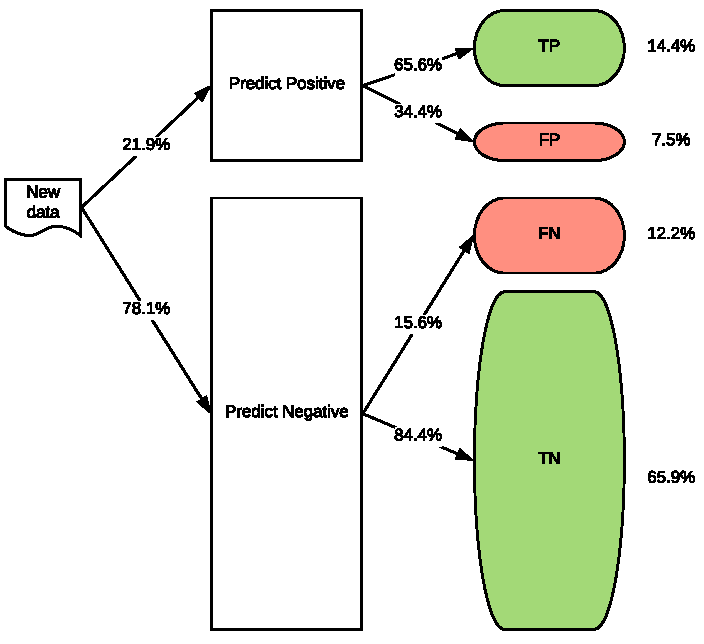
\includegraphics[width=5in]{classifier_flowchart}
\end{figure}

\noindent Note that \qu{new data} in the above illustration means data not used to construct $g$ and thus it means out of sample data.
\benum

%\subquestionwithpoints{4}  Approximate the future accuracy of $g$.\spc{0}

\subquestionwithpoints{3}  If we used this model to predict for $n^*=1,000$ new observations (sampled in the same fashion as the observations in $\mathbb{D}$), provide the confusion table for these predictions. Make sure you label the rows and columns appropriately. \spc{7}

\subquestionwithpoints{4} Which algorithm(s) could have produced $g$ \textit{directly}?

\begin{enumerate}[i)]
\item OLS
\item Logistic Regression
\item Perceptron
\item SVM
\item KNN
\item regression tree
\item classification tree
\item random forest
\end{enumerate}

\subquestionwithpoints{5} Assume this classifier was built using a probability estimation model with an imposed threshold. Mark this classifier's performance on an ROC curve and then draw an approximate \textit{example} ROC curve for different thresholds of this underlying probability estimation model as best as you can. Label the axes and important points on the axes. Also, plot the performance of \qu{random guessing} as a dotted line.\spc{11}

\subquestionwithpoints{2} Estimate the AUC of the ROC curve from (c).\spc{0}
\eenum


\pagebreak
\problem Consider the data generating process created by this \texttt{R} code:\\


\begin{lstlisting}
n = 1000
sigma = 0.2

x_t = 2 * pi
b = 3
xmin = 0
xmax = 4 * pi

x = runif(n, xmin, xmax)
f_x = sin(x) + b * ifelse(x > x_t, 1, 0)
delta = rnorm(n, 0, sigma)
y = f_x + delta
\end{lstlisting}

\noindent which is plotted here:

\begin{figure}[h]
\centering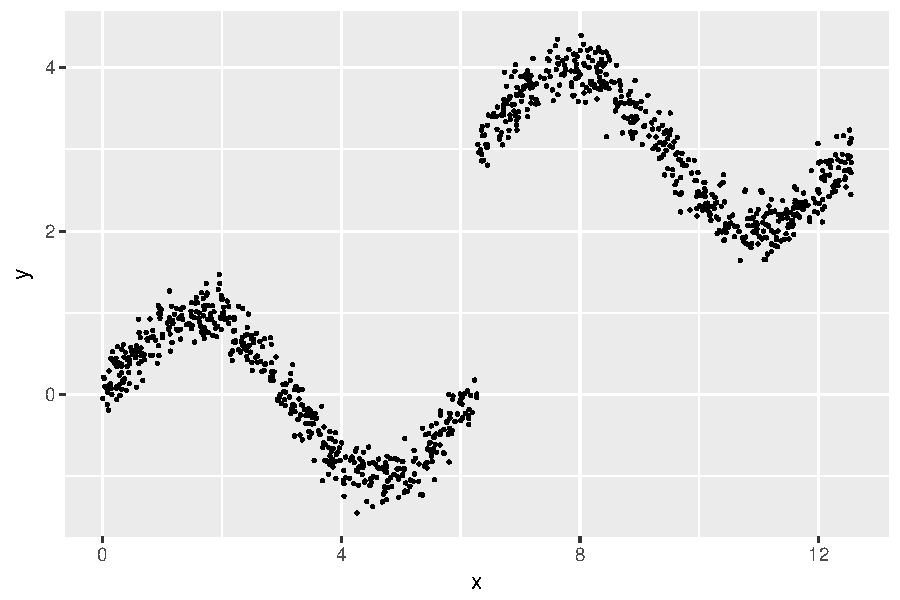
\includegraphics[width=7in]{wiggly}
\end{figure}

\noindent The goal is now to create a model $g$ using $x$ of this phenomenon $y$.
\clearpage

\benum

\subquestionwithpoints{5} In the underlined spaces below, rate each of the following algorithms in terms of the expected oos performance (where the $x^*$'s are sampled the same as in the code above) of the resultant $g$ where 1 indicates the \qu{best} performance, 2 indicates second-best performance, etc.

\begin{enumerate}[i)]
\item \line(1,0){20}~~ $\mathcal{A} =$ OLS where $\mathcal{H} = \braces{w_0 + w_1 x ~:~ \w \in \reals^2}$ 
%\item \line(1,0){20}~~ $\mathcal{A} =$ LS minimization using numerical methods where \\$\mathcal{H} = \braces{w_0 sin(w_1 x) ~:~ \w \in \reals^2}$ 
\item \line(1,0){20}~~  $\mathcal{A} =$ LS minimization using numerical methods  where \\$\mathcal{H} = \braces{w_0 + w_1 \indic{x \geq w_2} + w_3 sin(w_4 x) ~:~ \w \in \reals^5}$
\item \line(1,0){20}~~  $\mathcal{A} =$ a regression tree with $N_0 = 5$
\item \line(1,0){20}~~  $\mathcal{A} =$ a regression tree with $N_0 = 100$
\item \line(1,0){20}~~  $\mathcal{A} =$ a bag of trees with $T=1,001$ and default $N_0$
\item \line(1,0){20}~~  $\mathcal{A} =$ a random forest with $T=1,000$ and default $N_0$
\end{enumerate}~\\

The next few questions will be about drawing regression tree models for $y$. When drawing the trees, make sure inner nodes specify the split rule and leaf nodes specify the prediction value. Round to the nearest decimal.

\subquestionwithpoints{2} Draw a regression tree model with one node.\spc{3}

\subquestionwithpoints{4} Draw a regression tree model with three nodes.\spc{7}

\subquestionwithpoints{6} Draw a regression tree model with seven nodes and depth 2. Note that depth is defined as follows: the model in (b) has depth = 0 and the model in (c) has depth = 1 .\spc{8}


\eenum


\problem Recall the \texttt{adult} data where the phenomenon to model is whether someone has an income above or below \$50K based on the following features:

\begin{lstlisting}
pacman::p_load_gh("coatless/ucidata")
data(adult)
adult$native_country = NULL
adult$education_num = NULL
adult = na.omit(adult) #kill any observations with missingness
str(adult, vec.len = 2)
\end{lstlisting}

\vspace{-1cm}
\begin{verbatim}
'data.frame':	30161 obs. of  15 variables:
 $ age           : int  50 38 53 28 37 ...
 $ workclass     : Factor w/ 8 levels "Federal-gov",..: 6 4 4 4 4 ...
 $ fnlwgt        : int  83311 215646 234721 338409 284582 ...
 $ education     : Factor w/ 16 levels "10th","11th",..: 10 12 2 10 13 ...
 $ marital_status: Factor w/ 7 levels "Divorced","Married-AF-spouse",..: 3 1 3 3 3 ...
 $ occupation    : Factor w/ 14 levels "Adm-clerical",..: 4 6 6 10 4 ...
 $ relationship  : Factor w/ 6 levels "Husband","Not-in-family",..: 1 2 1 6 6 ...
 $ race          : Factor w/ 5 levels "Amer-Indian-Eskimo",..: 5 5 3 3 5 ...
 $ sex           : Factor w/ 2 levels "Female","Male": 2 2 2 1 1 ...
 $ capital_gain  : int  0 0 0 0 0 ...
 $ capital_loss  : int  0 0 0 0 0 ...
 $ hours_per_week: int  13 40 40 40 40 ...
 $ income        : Factor w/ 2 levels "<=50K",">50K": 1 1 1 1 1 ...
 - attr(*, "na.action")=Class 'omit'  Named int [1:2399] 14 27 38 51 61 ...
  .. ..- attr(*, "names")= chr [1:2399] "14" "27" ...
\end{verbatim}

\noindent Consider the model $g$ built with the following code:\\


\begin{lstlisting}
pacman::p_load_gh("coatless/ucidata")
data(adult)
adult = na.omit(adult) #kill any observations with missingness
adult_train = adult[sample(1 : nrow(adult), 2000), ]
y_train = adult_train$income
X_train = adult_train
X_train$income = NULL

options(java.parameters = "-Xmx8000m")
library(YARF)
mod_rf = YARF(X_train, y_train, num_trees = 500)
mod_rf
\end{lstlisting}

\noindent which generates the output:

\footnotesize
\begin{verbatim}
YARF initializing with a fixed 500 trees...
YARF factors created...
YARF after data preprocessed... 62 total features...
Beginning YARF classification model construction...done.
Calculating OOB error...done.
YARF v1.0 for classification
Missing data feature ON.
500 trees, training data n = 2000 and p = 61 
Model construction completed within 0.15 minutes.
OOB results on all observations as a confusion matrix:
             predicted <=50K predicted >50K model errors
actual <=50K        1379.000        107.000        0.072
actual >50K          207.000        307.000        0.403
use errors             0.131          0.258        0.157
\end{verbatim}
\normalsize

\benum

\subquestionwithpoints{3}  Approximate the future accuracy of $g$ when this model is used to predict \textit{on new data} (not on $\mathbb{D}$, the data used to build $g$) or write \qu{impossible} if this is not possible.\spc{10}

%\subquestionwithpoints{3}  Would this accuracy be higher or lower if $g$ was built using a bag of trees? Why?\spc{4}

Now instead build a model $g$ to estimate the probability of the income being greater than \$50K via the following code:\\

\begin{lstlisting}
logistic_mod = glm(income ~ ., adult_train, family = "binomial")
summary(logistic_mod)
\end{lstlisting}

which produces output

\footnotesize
\begin{verbatim}
                                      Estimate Std. Error z value Pr(>|z|)    
(Intercept)                         -8.253e+00  1.576e+00  -5.236 1.64e-07 ***
age                                  2.810e-02  6.856e-03   4.099 4.15e-05 ***
workclassLocal-gov                  -1.380e+00  4.708e-01  -2.931 0.003379 ** 
workclassPrivate                    -5.960e-01  3.659e-01  -1.629 0.103369    
workclassSelf-emp-inc               -5.986e-01  4.790e-01  -1.250 0.211410    
workclassSelf-emp-not-inc           -9.564e-01  4.290e-01  -2.230 0.025771 *  
workclassState-gov                  -1.372e+00  5.012e-01  -2.737 0.006202 ** 
fnlwgt                               6.514e-07  6.836e-07   0.953 0.340626    
education11th                        6.537e-01  8.483e-01   0.771 0.440961    
education12th                        4.499e-01  1.039e+00   0.433 0.665073    
education1st-4th                    -1.390e+01  5.747e+02  -0.024 0.980708    
education5th-6th                     1.194e+00  9.628e-01   1.240 0.214983    
education7th-8th                     3.006e-01  8.284e-01   0.363 0.716658    
education9th                        -2.640e-01  1.041e+00  -0.254 0.799712    
educationAssoc-acdm                  1.359e+00  7.424e-01   1.831 0.067103 .  
educationAssoc-voc                   1.420e+00  7.119e-01   1.995 0.046049 *  
educationBachelors                   2.080e+00  6.673e-01   3.118 0.001822 ** 
educationDoctorate                   3.257e+00  9.107e-01   3.576 0.000349 ***
educationHS-grad                     9.937e-01  6.487e-01   1.532 0.125548    
educationMasters                     2.382e+00  7.034e-01   3.386 0.000710 ***
educationPreschool                  -1.170e+01  2.400e+03  -0.005 0.996111    
educationProf-school                 2.474e+00  8.181e-01   3.024 0.002491 ** 
educationSome-college                1.033e+00  6.611e-01   1.562 0.118273    
marital_statusMarried-AF-spouse     -1.272e+01  2.400e+03  -0.005 0.995769    
marital_statusMarried-civ-spouse     2.588e+00  9.773e-01   2.648 0.008089 ** 
marital_statusMarried-spouse-absent -9.140e-01  1.208e+00  -0.757 0.449270    
marital_statusNever-married         -7.321e-01  3.628e-01  -2.018 0.043615 *  
marital_statusSeparated              3.013e-02  6.267e-01   0.048 0.961652    
marital_statusWidowed                6.004e-01  5.410e-01   1.110 0.267148    
occupationArmed-Forces              -1.495e+01  1.521e+03  -0.010 0.992157    
occupationCraft-repair               2.292e-01  3.248e-01   0.706 0.480422    
occupationExec-managerial            1.167e+00  3.135e-01   3.721 0.000199 ***
occupationFarming-fishing           -1.687e+00  6.912e-01  -2.440 0.014680 *  
occupationHandlers-cleaners         -1.572e-01  5.262e-01  -0.299 0.765177    
occupationMachine-op-inspct         -1.820e-01  4.010e-01  -0.454 0.649915    
occupationOther-service             -5.509e-01  4.297e-01  -1.282 0.199827    
occupationPriv-house-serv           -1.505e+01  7.301e+02  -0.021 0.983552    
occupationProf-specialty             1.127e+00  3.224e-01   3.496 0.000472 ***
occupationProtective-serv            1.301e+00  5.462e-01   2.382 0.017234 *  
occupationSales                      4.146e-01  3.317e-01   1.250 0.211377    
occupationTech-support               7.619e-01  4.645e-01   1.640 0.100981    
occupationTransport-moving           3.445e-01  4.262e-01   0.808 0.418942    
relationshipNot-in-family            1.218e+00  9.470e-01   1.286 0.198508    
relationshipOther-relative           1.256e+00  1.057e+00   1.188 0.234672    
relationshipOwn-child               -2.896e-01  8.605e-01  -0.337 0.736442    
relationshipUnmarried                1.188e+00  1.005e+00   1.183 0.237000    
relationshipWife                     1.854e+00  4.154e-01   4.462 8.13e-06 ***
raceAsian-Pac-Islander               6.805e-01  9.095e-01   0.748 0.454319    
raceBlack                            6.545e-01  8.464e-01   0.773 0.439366    
raceOther                           -1.397e+00  1.471e+00  -0.950 0.342290    
raceWhite                            9.463e-01  7.905e-01   1.197 0.231277    
sexMale                              7.514e-01  3.207e-01   2.343 0.019147 *  
capital_gain                         3.865e-04  4.631e-05   8.345  < 2e-16 ***
capital_loss                         8.257e-04  1.593e-04   5.183 2.19e-07 ***
hours_per_week                       2.198e-02  7.220e-03   3.045 0.002329 ** 
\end{verbatim}

\normalsize


\subquestionwithpoints{2} Let $p$ be the number of features after each categorical variable was dummied and a reference level dropped. How was this model fit? Choose the best answer below.

\begin{enumerate}[i)]
\item $\mathcal{A} = $ LS minimization with $\mathcal{H} = \braces{\w \cdot \x~:~ \w \in \reals^{p+1}}$
\item $\mathcal{A} = $ LS minimization with $\mathcal{H} = \braces{e^{\w \cdot \x}~:~ \w \in \reals^{p+1}}$
\item $\mathcal{A} = $ LS minimization with $\mathcal{H} = \braces{\frac{e^{\w \cdot \x}}{1 + e^{\w \cdot \x}}~:~ \w \in \reals^{p+1}}$
\item $\mathcal{A} = $ numerical methods to optimize maximum likelihood assuming independent Bernoulli r.v.'s for the $Y_1, \ldots, Y_n$ with $\mathcal{H} = \braces{\frac{e^{\w \cdot \x}}{1 + e^{\w \cdot \x}}~:~ \w \in \reals^{p+1}}$
\item $\mathcal{A} = $ numerical methods to optimize maximum likelihood assuming independent Normal r.v.'s for the $Y_1, \ldots, Y_n$ with $\mathcal{H} = \braces{\frac{e^{\w \cdot \x}}{1 + e^{\w \cdot \x}}~:~ \w \in \reals^{p+1}}$
\end{enumerate}

\subquestionwithpoints{6}  Interpret the estimate for \texttt{hours\_per\_week}. Round the estimate to two significant digits in your answer. \spc{9}


\subquestionwithpoints{4} For a given new person, the estimated probability of having an income over \$50K is $\hat{p} = 70\%$. What would be the probability estimate if this person was naturally observed with an \texttt{Exec-managerial} occupation instead of a \texttt{Adm-clerical} occupation? \spc{5}


\eenum



\problem Consider the following modeling exercise. The phenomenon is the grade on a comprehensive qualifying exam. The students taking the exam can take as long as they wish up to 5 hours (but most students finish well before the 5 hour limit). The maximum score on the exam is 100 and the minimum is 0. \\

We measure the amount of time students took to complete the exam in hours. On the next page is a scatterplot of $n=100$ students' grades and the duration of their exam.

\begin{figure}[h]
\centering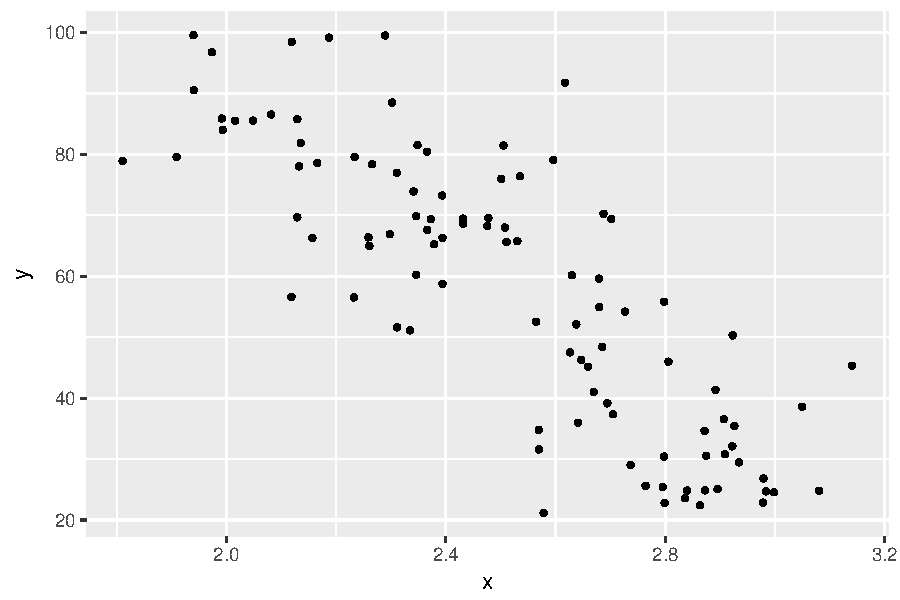
\includegraphics[width=6in]{time_and_grade}
\end{figure}

For the questions below, make reasonable common-sense assumptions about how this phenomenon would operate in the real world.

\benum

\subquestionwithpoints{2} Is time the students take to complete the exam associates with the students' grade? Yes / No.\spc{-0.7}
\subquestionwithpoints{2} Consider the answer to (a) to be \qu{yes} regardless of what you wrote for (a). Would this association be spurious? Yes / No.\spc{-0.7}
\subquestionwithpoints{2} Is time the students take to complete the exam a causal factor in the students' grade? Yes / No.\spc{-0.7}

\subquestionwithpoints{3} Write one sentence about you would test if the time the students take to finish the exam would be a causal factor of the students' grades.\spc{1}

\subquestionwithpoints{6} Draw an approximate causal diagram that includes both $x$ and $y$ and the casusal factors $z_1, z_2, \ldots$ (however many you wish) that would represent a situation where if the OLS regression $y \sim x + z_1 + z_2 + \ldots$ (as defined colloquially by a formula object in \texttt{R}) was fit, the coefficient on $x$ would be $\approx 0$. Make sure you describe \textit{in English} what your $z_1, z_2, \ldots$ measure in the real world. Use the convention that causes are drawn above effects. \spc{7}

\subquestionwithpoints{0} What would you do to improve this class for the students next year? Answer with regards to curriculum, assignments, presentation, theory vs. practice, etc.\spc{2}


\eenum


\end{document}


